\documentclass[11pt]{article}
\usepackage[hmargin=1in,vmargin=1in]{geometry}
\usepackage{xcolor}
\usepackage{amsmath,amssymb,amsfonts,url,sectsty,framed,tcolorbox,framed,graphicx}
\newcommand{\pf}{{\bf Proof: }}
\newtheorem{theorem}{Theorem}
\newtheorem{lemma}{Lemma}
\newtheorem{proposition}{Proposition}
\newtheorem{definition}{Definition}
\newtheorem{remark}{Remark}
\newcommand{\qed}{\hfill \rule{2mm}{2mm}}
\begin{document}
\noindent
\rule{\textwidth}{1pt}
\begin{center}
{\bf [CS304] Introduction to Cryptography and Network Security}
\end{center}
Course Instructor: Dr. Dibyendu Roy \hfill Winter 2022-2023 \\
Scribed by: Srushti Rathva (202051183) \hfill Lecture (Week 7) \\
\rule{\textwidth}{1pt}

\section*{Shift Rows}
Shift Rows : $\{0,1\}^{128} \rightarrow \{0,1\}^{128}$. \\
We're left shifting each $i^{th}$ row by $i$ positions. \\
\\
$
\begin{bmatrix}
\mathcal{S}_{00} & \mathcal{S}_{01} & \mathcal{S}_{02} & \mathcal{S}_{03} \\
\mathcal{S}_{10} & \mathcal{S}_{11} & \mathcal{S}_{12} & \mathcal{S}_{13} \\
\mathcal{S}_{20} & \mathcal{S}_{21} & \mathcal{S}_{22} & \mathcal{S}_{23} \\
\mathcal{S}_{30} & \mathcal{S}_{31} & \mathcal{S}_{32} & \mathcal{S}_{33} \\
\end{bmatrix}
_{4\times4}
\rightarrow
\begin{bmatrix}
\mathcal{S}_{00} & \mathcal{S}_{01} & \mathcal{S}_{02} & \mathcal{S}_{03} \\
\mathcal{S}_{11} & \mathcal{S}_{12} & \mathcal{S}_{13} & \mathcal{S}_{10}
\\
\mathcal{S}_{22} & \mathcal{S}_{23} & \mathcal{S}_{20} & \mathcal{S}_{21}
\\
\mathcal{S}_{33} & \mathcal{S}_{30} & \mathcal{S}_{31} & \mathcal{S}_{32}
\\
\end{bmatrix}
_{4\times4}
$ 

\section*{Mix Column}
Mix Column : $\{0,1\}^{128} \rightarrow \{0,1\}^{128}$. \\\\
$(\mathcal{S}_{ij})_{4\times4} \rightarrow (\mathcal{S}_{ij}^{'})_{4\times4} $ \\\\
Column = 
$ \begin{pmatrix}
\mathcal{S}_{0c} \\
\mathcal{S}_{1c} \\
\mathcal{S}_{2c} \\
\mathcal{S}_{3c} \\
\end{pmatrix} $ \\\\
For $i=0$ to $3$ \\
\hspace*{0.50cm} $t_{i}$ = Binary to Polynomial($\mathcal{S}_{ic}$) \\
\hspace*{0.50cm} $u_{0}$ = $[(x)t_{0} + (x+1)t_{1} + t_{2} + t_{3}]$ mod $(x^{8} + x^{4} + x^{3} + x + 1)$ \\
\hspace*{0.50cm} $u_{1}$ = $[(x)t_{1} + (x+1)t_{2} + t_{3} + t_{0}]$ mod $(x^{8} + x^{4} + x^{3} + x + 1)$ \\
\hspace*{0.50cm} $u_{2}$ = $[(x)t_{2} + (x+1)t_{3} + t_{0} + t_{1}]$ mod $(x^{8} + x^{4} + x^{3} + x + 1)$ \\
\hspace*{0.50cm} $u_{3}$ = $[(x)t_{3} + (x+1)t_{0} + t_{1} + t_{2}]$ mod $(x^{8} + x^{4} + x^{3} + x + 1)$ \\
$\mathcal{S'}_{ic}$ = Polynomial to Binary($u_{i}$) \\\\
$ \begin{pmatrix}
\mathcal{S}_{0c} \\
\mathcal{S}_{1c} \\
\mathcal{S}_{2c} \\
\mathcal{S}_{3c} \\
\end{pmatrix} 
\xrightarrow{MixColumn}
\begin{pmatrix}
\mathcal{S'}_{0c} \\
\mathcal{S'}_{1c} \\
\mathcal{S'}_{2c} \\
\mathcal{S'}_{3c} \\
\end{pmatrix}
$ \\
\\\\
$ \begin{bmatrix}
x & x+1 & 1 & 1 \\
1 & x & x+1 & 1 \\
1 & 1 & x & x+1 \\
x+1 & 1 & 1 & x \\
\end{bmatrix} 
\begin{bmatrix}
\mathcal{S}_{00} & \mathcal{S}_{01} & \mathcal{S}_{02} & \mathcal{S}_{03} \\
\mathcal{S}_{10} & \mathcal{S}_{11} & \mathcal{S}_{12} & \mathcal{S}_{13} \\
\mathcal{S}_{20} & \mathcal{S}_{21} & \mathcal{S}_{22} & \mathcal{S}_{23} \\
\mathcal{S}_{30} & \mathcal{S}_{31} & \mathcal{S}_{32} & \mathcal{S}_{33} \\
\end{bmatrix}
mod(x^{8} + x^{4} + x^{3} + x + 1)
=
\begin{bmatrix}
\mathcal{S'}_{00} & \mathcal{S'}_{01} & \mathcal{S'}_{02} & \mathcal{S'}_{03} \\
\mathcal{S'}_{10} & \mathcal{S'}_{11} & \mathcal{S'}_{12} & \mathcal{S'}_{13} \\
\mathcal{S'}_{20} & \mathcal{S'}_{21} & \mathcal{S'}_{22} & \mathcal{S'}_{23} \\
\mathcal{S'}_{30} & \mathcal{S'}_{31} & \mathcal{S'}_{32} & \mathcal{S'}_{33} \\
\end{bmatrix}
$ \\
\\\\
$ \begin{bmatrix}
2 & 3 & 1 & 1 \\
1 & 2 & 3 & 1 \\
1 & 1 & 2 & 3 \\
3 & 1 & 1 & 2 \\
\end{bmatrix} 
\begin{bmatrix}
\mathcal{S}_{00} & \mathcal{S}_{01} & \mathcal{S}_{02} & \mathcal{S}_{03} \\
\mathcal{S}_{10} & \mathcal{S}_{11} & \mathcal{S}_{12} & \mathcal{S}_{13} \\
\mathcal{S}_{20} & \mathcal{S}_{21} & \mathcal{S}_{22} & \mathcal{S}_{23} \\
\mathcal{S}_{30} & \mathcal{S}_{31} & \mathcal{S}_{32} & \mathcal{S}_{33} \\
\end{bmatrix}
mod(x^{8} + x^{4} + x^{3} + x + 1)
=
\begin{bmatrix}
\mathcal{S'}_{00} & \mathcal{S'}_{01} & \mathcal{S'}_{02} & \mathcal{S'}_{03} \\
\mathcal{S'}_{10} & \mathcal{S'}_{11} & \mathcal{S'}_{12} & \mathcal{S'}_{13} \\
\mathcal{S'}_{20} & \mathcal{S'}_{21} & \mathcal{S'}_{22} & \mathcal{S'}_{23} \\
\mathcal{S'}_{30} & \mathcal{S'}_{31} & \mathcal{S'}_{32} & \mathcal{S'}_{33} \\
\end{bmatrix}
$ \\\\
\\
MixColumn($\mathcal{S}$) = $M\mathcal{S}$ \\
MixCoulmn(MixCoulmn(MixCoulmn(MixCoulmn($\mathcal{S}$)))) = $M^{4}\mathcal{S}$ \\
\hspace*{9.45cm} = $I\mathcal{S}$ \hspace{3cm}
$\because M^{4} = I$

\section*{Key Scheduling Algorithm}
Input : 128 bit Key \\
Output : 11 Round keys each of length 128 bits \\
We'll compute 44 words denoted by w[0],w[1]... w[43] \\\\
\textbf{Rotword}\\
f($B_{0},B_{1},B_{2},B_{3}$) = ($B_{1},B_{2},B_{3},B{0}$) \\\\
\textbf{Subword}\\
f($B_{0},B_{1},B_{2},B_{3}$) = ($B'_{0},B'_{1},B'_{2},B'_{3}$) where $B'_{i}$ = Subbyte($B_{i}$) \\\\
\textbf{10 Round Constants }\\
Rcon[1] = 01000000 \\
Rcon[2] = 02000000 \\
Rcon[3] = 04000000 \\
Rcon[4] = 08000000 \\
Rcon[5] = 10000000 \\
Rcon[6] = 20000000 \\
Rcon[7] = 40000000 \\
Rcon[8] = 80000000 \\
Rcon[9] = 1B000000 \\
Rcon[10] = 36000000 \\
\\
\textbf{Algorithm}\\
For $i=0$ to $3$ \\
\hspace*{0.50cm} w[i] = (Key[4i], Key[4i+1], Key[4i+2], Key[4i+3]) \\\\
For $i=4$ to $43$ \\
\hspace*{0.50cm} temp = w[i-1] \\
\hspace*{0.50cm} If i $\equiv$ 0 mod 4 \\
\hspace*{1cm} temp = SUBWORD(ROTWORD(temp)) $\oplus$ Rcon[i/4] \\
\hspace*{0.50cm} w[i] = w[i-4] $\oplus$ temp  \\\\
return(w[0], w[1], ... w[43]) \\
\\
\textbf{Round Keys}\\
$K_{1}$ = w[0] $\|$ w[1] $\|$ w[2] $\|$ w[3] \\
$K_{2}$ = w[4] $\|$ w[5] $\|$ w[6] $\|$ w[7]  \\
\vdots \\
$K_{11}$ = w[40] $\|$ w[41] $\|$ w[42] $\|$ w[43] \\

\section*{Modes of Operation}
\begin{enumerate}
\itemsep-0.5em 
\item Electronic Code Book Mode
\item Cipher Feedback Mode
\item Cipher Block Chaining Mode
\item Output Feedback Mode
\item Counter Mode
\item Counter with Cipher Block Chaining Mode
\end{enumerate}

\subsection*{Electronic Codebook Mode (ECB)}
\textbf{Encryption} \\
C = $c_{0} \| c_{1} \| ... \| c_{t}$ \\
$c_{i} = Enc(m_{i},K)$ \hspace{1cm} $\forall i\in [0,t]$ \\
\\
\textbf{Decryption} \\
M = $m_{0} \| m_{1} \| ... \| m_{t}$ \\
$m_{i} = Dec(c_{i},K)$ \hspace{1cm} $\forall i\in [0,t]$ \\
\begin{center}
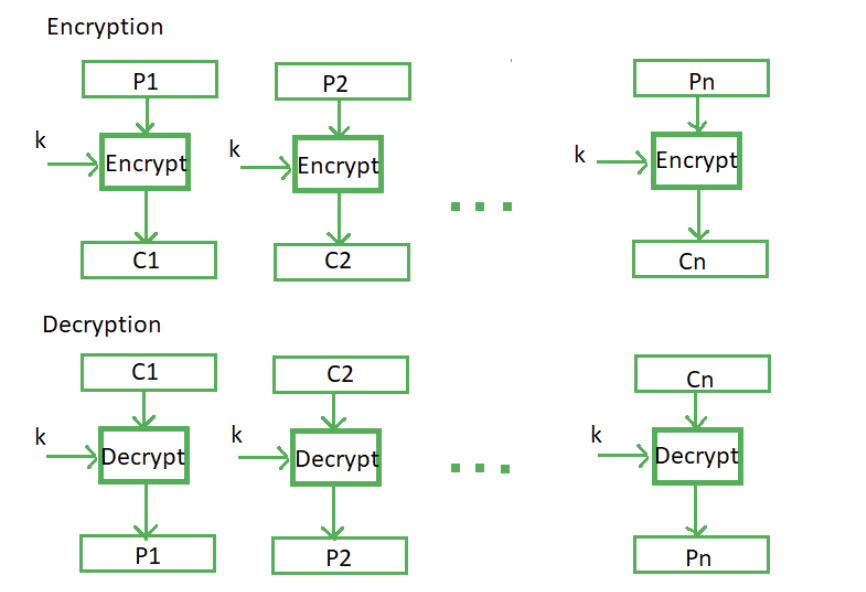
\includegraphics[width=300pt]{p1.png} \\  
\end{center}
This mode can be implemented parallelly but if $m_{i} = m_{j}$ then $c_{i} = c_{j}$ 

\subsection*{Cipher Block Chaining Mode (CBC)}
\textbf{Encryption} \\
C = $c_{0} \| c_{1} \| ... \| c_{t}$ \\
$IV \rightarrow$ Initialization Vector \\
$c_{0} = IV $ \\
$c_{i} = Enc(c_{i-1} \oplus m_{i},K)$ \hspace{1cm} $\forall i\in [1,t]$ \\\\
\textbf{Decryption} \\
M = $m_{0} \| m_{1} \| ... \| m_{t}$ \\
$IV \rightarrow$ Initialization Vector \\
$c_{0} = IV $ \\
$m_{i} = Dec(c_{i},K) \oplus c_{i-1}$ \hspace{1cm} $\forall i\in [1,t]$ \\
\begin{center}
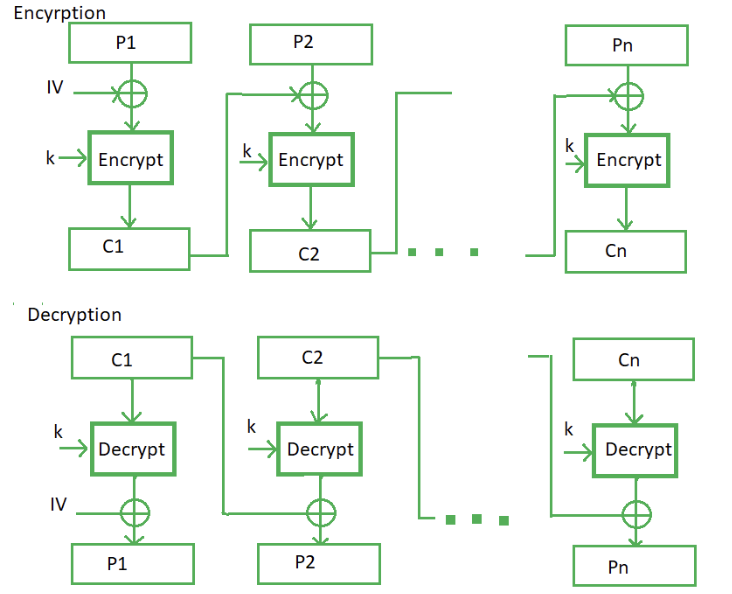
\includegraphics[width=300pt]{p2.png} \\  
\end{center}
\section*{Hash Function}
$h$ : A $\rightarrow$ B \\
$h(X) = Y$ \\
1. If $X$ is altered to $X'$ then $h(X)$ will be completely different from $h(X')$ \\
2. Given $Y$, it is practically infeasible to find $X$ such that $h(X) = Y$\\
3. Given $X$ and $Y$, it is practically infeasible to find $X'$ such that $h(X) = h(X')$\\
\\
\textbf{Alice} \hspace{6.5cm} \textbf{Bob} \\
$X = E(M,K)\xrightarrow{\hspace*{2.5cm}X\hspace*{2.5cm}} X_{1} = D(X',K)$ \\
$S_{1} = h(M,K)\xrightarrow{\hspace*{2.5cm}S_{1}\hspace*{2.5cm}} S_{2}$ \\
If $ h(M,K) = S_{2}$ then Bob accepts $X_{1}$. 
\subsection*{Hash Family}
It is a four tuple $(P,S,K,H)$ satisfying following conditions : \\
1. P is the set of all possible messages. \\
2. S is the set of all possible message digests or authentication tags. \\
3. K is the key space
4. For each $k_{i} \in$ K there is a hash function $h_{k_{1}} \in$ H such that,\\
$h_{k_{1}}$ : P $\rightarrow$ S \\
$|P| \geq |S|$, More specifically $|P| \geq 2|S| $ 
\begin{center}
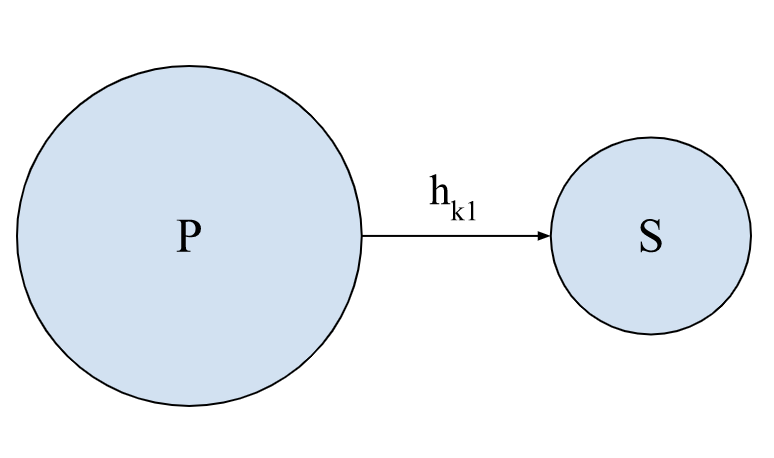
\includegraphics[width=200pt]{p3.png}
\end{center}
\textbf{Keyed Hash Function}\\
If the key is involved in computing hash value then the hash function is called Keyed Hash Function. \\\\
\textbf{Unkeyed Hash Function}\\
If the key is not involved in computing hash value then the hash function is called Keyed Hash Function.
\subsection*{Preimage Finding Problem}
$h$ : P $\rightarrow$ S \\
Given $Y \in$ S, Find $X \in$ P such that $h(X) = Y$ \\
\\
For a hash function $h$ if you can not find preimage in feasible time than the $h$ is called \textbf{preimage resistant function}.
\subsection*{Second Preimage Finding Problem}
$h$ : P $\rightarrow$ S \\
Given $X \in$ P and $h(X)$, Find $X' \in$ P such that $X \neq X'$ and $h(X) = h(X')$ \\
\\
For a hash function $h$ if you can not find second preimage in feasible time than the $h$ is called \textbf{second preimage resistant function}.
\subsection*{Collision Finding Problem}
$h$ : P $\rightarrow$ S \\
Find $X,X' \in$ P such that $X \neq X'$ and $h(X) = h(X')$ \\
\\
For a hash function $h$ if you can not find the pair in feasible time than the $h$ is called \textbf{collision resistant function}.
\subsection*{Ideal Hash Function}
Let, $h$ : P $\rightarrow$ S \\
$h$ is called Ideal hash function if given $X \in$ P, for finding $h(X)$ either one has to apply $h$ on $X$ or look in the hash table.
\subsection*{Preimage Finding Algorithm}
$h$ : $X \rightarrow Y$ \\\\
Choose any $X_{o} \subseteq X$ such that $|X_{o}| = Q$ \\
\hspace*{1.4cm}for each $x \in X_{o}$ \\
\hspace*{2cm}compute $y_{x} = h(x)$ \\
\hspace*{2cm}if $y_{x} = y$ \\
\hspace*{2.5cm}return $x$ \\\\
Time Complexity : $O(Q)$ \\\\
$X_{o} = \{x_{1},x_{2},...,x_{Q}\}$\\
$E_{i}$ : Event $h(x_{i}) = y$, \hspace{1cm} $1 \leq i \leq Q$\\\\
Pr[$E_{i}$] = $\frac{1}{M}$ \\\\
Pr[$E_{i}^{c}$] = 1- $\frac{1}{M}$  \\\\
Pr[$E_{1} \cup E_{2} \cup E_{3} \cup ... \cup E_{Q}$] = 1 - Pr[$E_{1}^{c} \cap E_{2}^{c} \cap E_{3}^{c} \cap ... \cap E_{Q}^{c}$] \\\\
\hspace*{4.55cm} = 1 - $ \Pi_{i=1}^{Q}$ Pr[$E_{i}^{c}$] \\\\
\hspace*{4.55cm} = 1 - $(1- \frac{1}{M})^{Q}$ \\\\
\hspace*{4.55cm} $\approx 1 - (1- \binom Q1 \frac{1}{M})^{Q}$ \\\\
\hspace*{4.55cm} = $\frac{Q}{M}$
\end{document}
